%iffalse
\let\negmedspace\undefined
\let\negthickspace\undefined
\documentclass[journal,12pt,onecolumn]{IEEEtran}
\usepackage{cite}
\usepackage{amsmath,amssymb,amsfonts,amsthm}
\usepackage{algorithmic}
\usepackage{graphicx}
\usepackage{textcomp}
\usepackage{xcolor}
\usepackage{txfonts}
\usepackage{listings}
\usepackage{enumitem}
\usepackage{mathtools}
\usepackage{pgfplots}
\usepackage{gensymb}
\usepackage{comment}
\usepackage[breaklinks=true]{hyperref}
\usepackage{tkz-euclide} 
\usepackage{listings}
\usepackage{gvv}                                        
%\def\inputGnumericTable{}                                 
\usepackage[latin1]{inputenc}                                
\usepackage{color}                                            
\usepackage{array}                                            
\usepackage{longtable}                                       
\usepackage{calc}                                             
\usepackage{multirow}                                         
\usepackage{hhline}                                           
\usepackage{ifthen}                                           
\usepackage{lscape}
\usepackage{tabularx}
\usepackage{array}
\usepackage{float}

\usepackage{enumitem}
\usepackage{xcolor}
%\usepackage{multicol}


\newtheorem{theorem}{Theorem}[section]
\newtheorem{problem}{Problem}
\newtheorem{proposition}{Proposition}[section]
\newtheorem{lemma}{Lemma}[section]
\newtheorem{corollary}[theorem]{Corollary}
\newtheorem{example}{Example}[section]
\newtheorem{definition}[problem]{Definition}
\newcommand{\BEQA}{\begin{eqnarray}}
\newcommand{\EEQA}{\end{eqnarray}}
\newcommand{\define}{\stackrel{\triangle}{=}}
\theoremstyle{remark}
\newtheorem{rem}{Remark}

\title{2009-PH-1-12}
\author{AI24BTECH11023 - Tarun Reddy Pakala}
\begin{document}
\bibliographystyle{IEEEtran}

\maketitle
\bigskip
\renewcommand{\thefigure}{\theenumi}
\renewcommand{\thetable}{\theenumi}
\begin{enumerate}
    \item The value of the contour integral, $\abs{\int_{C} \overrightarrow{r} \times d\overrightarrow{\theta} \, }$, for a circle $C$ of radius $r$ with center at origin is
    \begin{enumerate}
    \item $2\pi r$
    \item $r^2/2$
    \item $\pi r^2$
    \item $r$
    \end{enumerate}
    \item An electrostatic field $\overrightarrow{E}$ exists in a given region R. Choose the WRONG statement.
    \begin{enumerate}
    \item Circulation of $\overrightarrow{E}$ is zero
    \item $\overrightarrow{E}$ can always be expressed as the gradient of a scalar field
    \item The potential difference between any two arbitrary points in the region R is zero
    \item The work  done in a closed path lying entirely in R is zero
    \end{enumerate}
    \item The Lagrangian of a free particle in spherical polar co-ordinates is given by $L = \frac{1}{2} m \left( \dot{r}^2 + r^2 \dot{\theta}^2 + r^2 \dot{\phi}^2 \sin^2 \theta \right)$. The quantity that is conserved is
    \begin{enumerate}
    \item $\frac{\partial L}{\partial \dot{r}}$
    \item $\frac{\partial L}{\partial \dot{\theta}}$
    \item $\frac{\partial L}{\partial \dot{\phi}}$
    \item $\frac{\partial L}{\partial \dot{\phi}} + \dot{r} \dot{\theta}$
    \end{enumerate}
    \item A conducting loop $L$ of surface area $S$ is moving with a velocity $\overrightarrow{v}$ in a magnetic field $\overrightarrow{B}(\overrightarrow{r},t)$=$\overrightarrow{B_0}t^2$, $B_o$ is a positive constant of suitable dimensions. The emf induced, $V_{emf}$, in the loop is given by
    \begin{enumerate}
        \item -$\int_S \frac{\partial \overrightarrow{B}}{\partial t} \cdot d\overrightarrow{S}$
        \item $\oint_L (\overrightarrow{v} \times \overrightarrow{B}) \cdot d\overrightarrow{L}$
        \item -$\int_S \frac{\partial \overrightarrow{B}}{\partial t} \cdot d\overrightarrow{S}$-$\oint_L (\overrightarrow{v} \times \overrightarrow{B}) \cdot d\overrightarrow{L}$
        \item -$\int_S \frac{\partial \overrightarrow{B}}{\partial t} \cdot d\overrightarrow{S}$+$\oint_L (\overrightarrow{v} \times \overrightarrow{B}) \cdot d\overrightarrow{L}$
    \end{enumerate}
    \item The eigenvalues of the matrix $A= 
\begin{bmatrix}
0 & i \\
i & 0
\end{bmatrix}
$ are
    \begin{enumerate}
    \item real and distinct
    \item complex and distinct
    \item complex and coinciding
    \item real and coinciding
    \end{enumerate}
    \item $\sigma_i(i=1, 2, 3)$ represent the Pauli spin matrices. Which one of the following is NOT true ?
    \begin{enumerate}
        \item $\sigma_i \sigma_j$+$\sigma_j \sigma_i$=2$\delta_{ij}$
        \item $Tr(\sigma_i)=0$
        \item The eigenvalues of $\sigma_i$ are $\pm1$
        \item det($\sigma_i$)=1
    \end{enumerate}
    \item Which one of the functions given below represents the bound state eigenfunction of the operator $ - \frac{d^2}{dx^2} $ in the region, $0 \leq x < \infty$ with the eigenvalue -4 ? 
    \begin{enumerate}
    \item $A_o e^{2x}$
    \item $A_o \cosh{2x}$
    \item $A_o e^{-2x}$
    \item $A_o \sinh{2x}$
    \end{enumerate}
    \item Pick the WRONG statement.
    \begin{enumerate}
        \item The nuclear force is independent of electric charge
        \item The Yukawa potential is proportional to $r^{-1} \exp\left(\frac{mc}{\hbar} r\right)$, where $r$ is the separation between two nucleons
        \item The range of nuclear force is order of $10^{-15}m-10^{-14}m$
        \item The nucleons interact among each other by the exchange of mesons
    \end{enumerate}
    \item If $p$ and $q$ are the position and momentum variables, which one of the following is NOT a canonical transformation ?
    \begin{enumerate}
        \item $Q=\alpha q$ and $P= \frac{1}{\alpha}p$, for $\alpha \neq 0$
        \item $Q=\alpha q+\beta p$ and $P=\beta q+\alpha p$ for $\alpha,\beta$ real and $\alpha^2-\beta^2=1$
        \item $Q=p$ and $P=q$
        \item $Q=p$ and $P=-q$
    \end{enumerate}
    \item The Common Mode Rejection Ratio (CMRR) of a differential amplifier using an operational amplifier is 100 dB. The output voltage for a differential input of 200 $\mu$V is 2 V. The common mode gain is
    \begin{enumerate}
        \item 10
        \item 0.1
        \item 30 dB
        \item 10 dB
    \end{enumerate}
    \item In an insulating solid which one of the following physical phenomena is a consequence of Pauli's exclusion principle ?
    \begin{enumerate}
        \item Ionic conductivity
        \item Ferromagnetism
        \item Paramagnetism
        \item Ferroelectricity
    \end{enumerate}
    \item Which one of the following curves gives the solution of the differential equation $k_1 \frac{dx}{dt} + k_2 x = k_3$, where $k_1,k_2$ and $k_3$ are positive constants with initial conditions $x=0$ at $t=0$ ?
    \begin{enumerate}
        \item 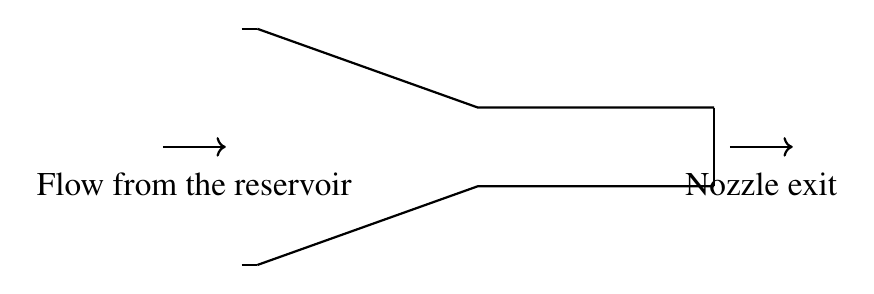
\begin{tikzpicture}
    % Draw the nozzle shape with short vertical lines at the opening
    \draw[thick] (-3,1.5) -- (-2.8,1.5);
    \draw[thick] (-3,-1.5) -- (-2.8,-1.5);
    \draw[thick] (-2.8,1.5) -- (0,0.5) -- (3,0.5);
    \draw[thick] (-2.8,-1.5) -- (0,-0.5) -- (3,-0.5);
    
    % Vertical line at the nozzle exit
    \draw[thick] (3,0.5) -- (3,-0.5);

    % Flow direction arrows
    \draw[->, thick] (-4,0) -- (-3.2,0);
    \draw[->, thick] (3.2,0) -- (4,0);

    % Labels for the flow and nozzle exit, placed below arrows
    \node[below] at (-3.6,-0.2) {\large Flow from the reservoir};
    \node[below] at (3.6,-0.2) {\large Nozzle exit};
\end{tikzpicture}

	\item \begin{figure}[!ht]
\centering
\resizebox{3cm}{3cm}{%
\begin{circuitikz}
\tikzstyle{every node}=[font=\LARGE]
\draw [ line width=0.6pt](2.75,12) to[sinusoidal voltage source, sources/symbol/rotate=auto] (3.25,11.5);
\draw [ line width=0.6pt](3.25,11.75) to[european resistor] (9.5,11.75);
\draw [line width=0.6pt, ->, >=Stealth] (9.5,11.75) -- (9.5,11);
\draw [ line width=0.6pt](4,12.25) to[short] (4,11.25);
\draw [ line width=0.6pt](4,11.5) to[short] (4,11);
\draw [ line width=0.6pt](8.75,12.25) to[short] (8.75,11);
\draw [ line width=0.6pt](4,11.25) to[short] (4.5,11.25);
\draw [ line width=0.6pt](8.75,11.25) to[short] (8.25,11.25);
\draw [ line width=0.6pt](4.25,11.25) to[short] (5.25,11.25);
\draw [ line width=0.6pt](8.25,11.25) to[short] (7.25,11.25);
\draw [ line width=0.6pt](5,11.25) to[european resistor] (5,8.5);
\draw [ line width=0.6pt](7.5,11.25) to[european resistor] (7.5,8.5);
\draw [ line width=0.6pt](4.75,8.5) to[short] (8,8.5);
\draw [line width=0.6pt, ->, >=Stealth] (6.25,8.5) -- (6.25,7.75);
\node [font=\normalsize] at (6.75,8) {Bus 3};
\node [font=\normalsize] at (4,12.5) {Bus 1};
\node [font=\normalsize] at (8.75,12.5) {Bus 2};
\node [font=\normalsize] at (6.25,12.25) {j q};
\node [font=\normalsize] at (4.5,10) {j r};
\node [font=\normalsize] at (8.25,9.75) {j p};
\end{circuitikz}
}%

\label{fig:my_label}
\end{figure}

	\item \begin{figure}[!ht]
\centering
\resizebox{3cm}{3cm}{%
\begin{circuitikz}
\tikzstyle{every node}=[font=\small]
\draw (4.25,12.25) to[battery1] (4.25,7.75);
\draw (4.25,12.25) to[short] (6.25,12.25);
\draw (4.25,7.75) to[short] (6.25,7.75);
\draw (6.25,12.25) to[R] (6.25,10.25);
\draw (6.25,10.25) to[R] (6.25,7.75);
\draw (6.25,10.25) to[short] (8.75,10.25);
\draw (6.25,7.75) to[short] (8.75,7.75);
\draw (8.75,7.75) to[R] (8.75,9.25);
\draw (8.75,10.25) to[D] (8.75,9);
\node [font=\small] at (4,10.25) {+};
\node [font=\small] at (4,9.75) {-};
\node [font=\small] at (4.75,10.5) {24 Volt};
\node [font=\small] at (6.75,11.25) {12 k$\Omega$};
\node [font=\small] at (6.75,9) {6 k$\Omega$};
\node [font=\small] at (8,8.5) {3.3 k$\Omega$};
\end{circuitikz}
}%

\label{fig:my_label}
\end{figure}
 
	\item \begin{figure}[H]
\centering
\resizebox{3cm}{3cm}{%
\begin{circuitikz}
\tikzstyle{every node}=[font=\small]
\draw [->, >=Stealth] (3.5,10.75) -- (3.5,13.75);
\draw [->, >=Stealth] (3.5,10.75) -- (10.75,10.75);
\draw [->, >=Stealth] (2.25,10.75) -- (3.25,10.75);
\draw [dashed] (4.5,13.25) -- (4.5,8.25);
\draw [dashed] (7.25,13.25) -- (7.25,8.25);
\draw [dashed] (10,13.25) -- (10,8.25);
\draw [dashed] (2,8.25) -- (10,8.25);
\draw [dashed] (2,13) -- (10,13);
\draw [short] (4.5,10.75) -- (7.25,11.75);
\draw [short] (7.25,11.75) -- (10,9.75);
\draw [short] (4.5,10.75) -- (10,9.75);
\node [font=\small] at (2.5,11) {$M>1$};
\node [font=\small] at (3.5,14) {$y$};
\node [font=\small] at (11,10.75) {$x$};
\node [font=\small] at (4.5,8) {$X_A$};
\node [font=\small] at (7.25,8) {$X_B$};
\node [font=\small] at (10,8) {$X_C$};
\node [font=\small] at (1.75,8.25) {$Y_{II}$};
\node [font=\small] at (1.75,13) {$Y_I$};
\node [font=\small] at (5.5,11) {$\alpha$};
\node [font=\small] at (6.5,10.5) {$\alpha$};
\node [font=\small] at (9,10) {$2\alpha$};
\end{circuitikz}
}%
\label{fig:my_label}
\end{figure}


    \end{document}
